% !TEX root = ../main.tex

% 实验记录	
\begin{table}
	\renewcommand\arraystretch{1.7}
	\centering
	\begin{tabularx}{\textwidth}{|X|X|X|X|}
		\hline
		Major: & Physics & Grade: & 2022 \\
		\hline
		Name: & 杨舒云 \& 戴鹏辉 & Student number: & 22344020 \& 22344016\\
		\hline
		Room temperature: & 30\degree C & Experimental location: & A522 \\
		\hline
		Student's Signature:& \textbf{In Attachment} & Score: &\\
		\hline
		Experiment time:& 2024/9/25 & Teacher's Signature:&\\
		\hline
	\end{tabularx}
\end{table}
\section{ET2-1 Welding and Debugging of Bluetooth Speakers \\  Experimental Record}


%---------------------------------------------------------------------
% 实验过程记录
\subsection{Content, Procedures \& Results}

% 操作步骤
\subsubsection{Operations}
\begin{enumerate}
	\item According to the instructions, complete the welding of the Bluetooth speaker circuit and the assembly of the speaker as a whole. The following is a description of the welding process:
		\begin{enumerate}
			\item Solder the components one by one in the order shown in the tutorial.
			\item It is important to note that some components have positive and negative electrodes, and the direction cannot be wrong. Usually the long foot represents the positive pole.
			\item During the welding process, make sure to wear appropriate protective equipment, control the temperature and time, clean the solder joint and use the right amount of solder, and check the quality of the solder joint after welding to ensure the safety and quality of the welding.
		\end{enumerate}
	\item Measure the closed-loop gain of the power amplifier section of the Bluetooth speaker circuit.
	\item Finally, we referred to the soldered Bluetooth speaker circuit and PCB, taught ourselves KICAD, and copied the PCB.
\end{enumerate}	

% 实验结果
\subsubsection{Display}

We measured the output voltage variation with input voltage at a fixed frequency of 1kHz and the output voltage variation with frequency at a fixed input voltage of 50.0Vrms.

The results are shown in \cref{tab:tab1} and \cref{tab:tab2}.

\begin{table}[htbp]
	\centering
	\begin{tabular}{|c|c|c|c|c|c|c|c|c|c|c|}
		\hline
		\( u_{in} \)/mVrms & 10.0 & 20.0 & 30.0 & 40.0 & 50.0 & 60.0 & 70.0 & 80.0 & 90.0 & 100.0 \\
		\hline
		\( u_{out} \)/mVrms & 80.1 & 159.5 & 239.1 & 320.0 & 400.1 & 480.5 & 560.5 & 640.5 & 720.7 & 800.0 \\
		\hline
	\end{tabular}
	\caption{The output voltage variation with input voltage at a fixed frequency of 1kHz}
	\label{tab:tab1}
\end{table}

\begin{table}[htbp]
	\centering
	\begin{tabular}{|c|c|c|c|c|c|c|c|c|}
		\hline
		frequency/Hz & 20 & 35 & 70 & 100 & 200 & 500 & 700 & 1000 \\
		\hline
		\( u_{out} \)/Vrms & 187.4 & 271.9 & 351.9 & 374.4 & 393.6 & 399.9 & 400.6 & 400.9 \\
		\hline
	\end{tabular}
	\caption{The output voltage variation with frequency at a fixed input voltage of 50.0Vrms}
	\label{tab:tab2}
\end{table}

As requested by the teacher, we did not measure the power gain, but we conducted a theoretical analysis, see the data \textbf{analysis} section for details.

PCB:

After class, we used KiCAD and tried to copy the PCB drawing by referring to the datasheet of LM4863 chip and the schematic diagram of Bluetooth speaker, as shown in the \cref{fig:fig-PCB}.

\begin{figure}[htbp]
	\centering
	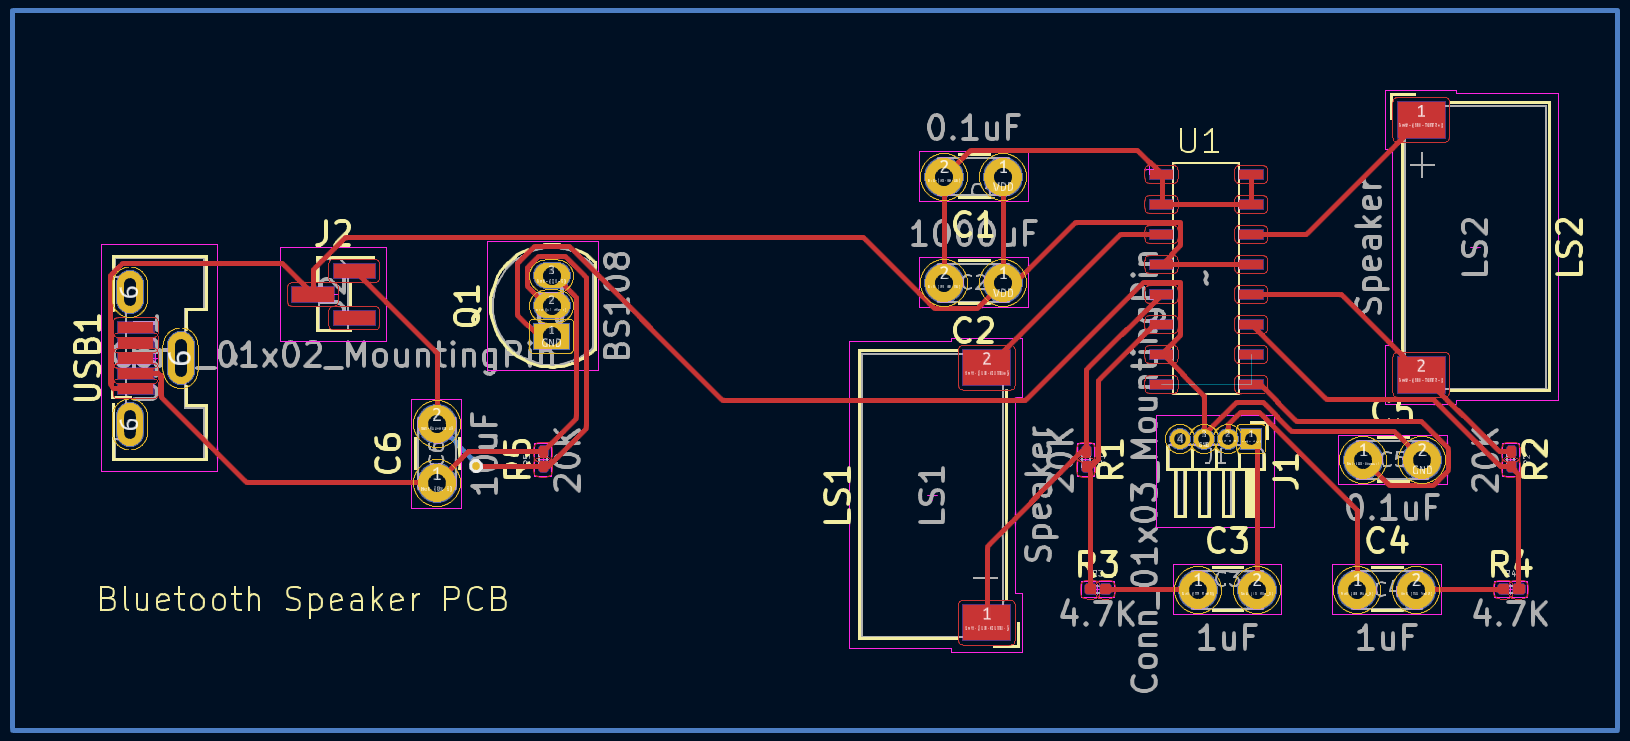
\includegraphics[width=0.8\textwidth]{ET2_1_PCB.png}
	\caption{PCB drawing}
	\label{fig:fig-PCB}
\end{figure}


%---------------------------------------------------------------------
% 原始数据
\clearpage
\subsection{Original Data}
The original data in the experimental notebook is shown in \cref{fig:fig-o} (signed).

\begin{figure}[htbp]
	\centering
	\includegraphics[width=0.6\textwidth]{ET2_1_original_data.jpg}
	\caption{Original data}
	\label{fig:fig-o}
\end{figure}

\clearpage
The welded and assembled Bluetooth speaker is shown in the \cref{fig:finished_product1} and \cref{fig:finished_product2}.

\begin{figure}[htbp]
	\centering
	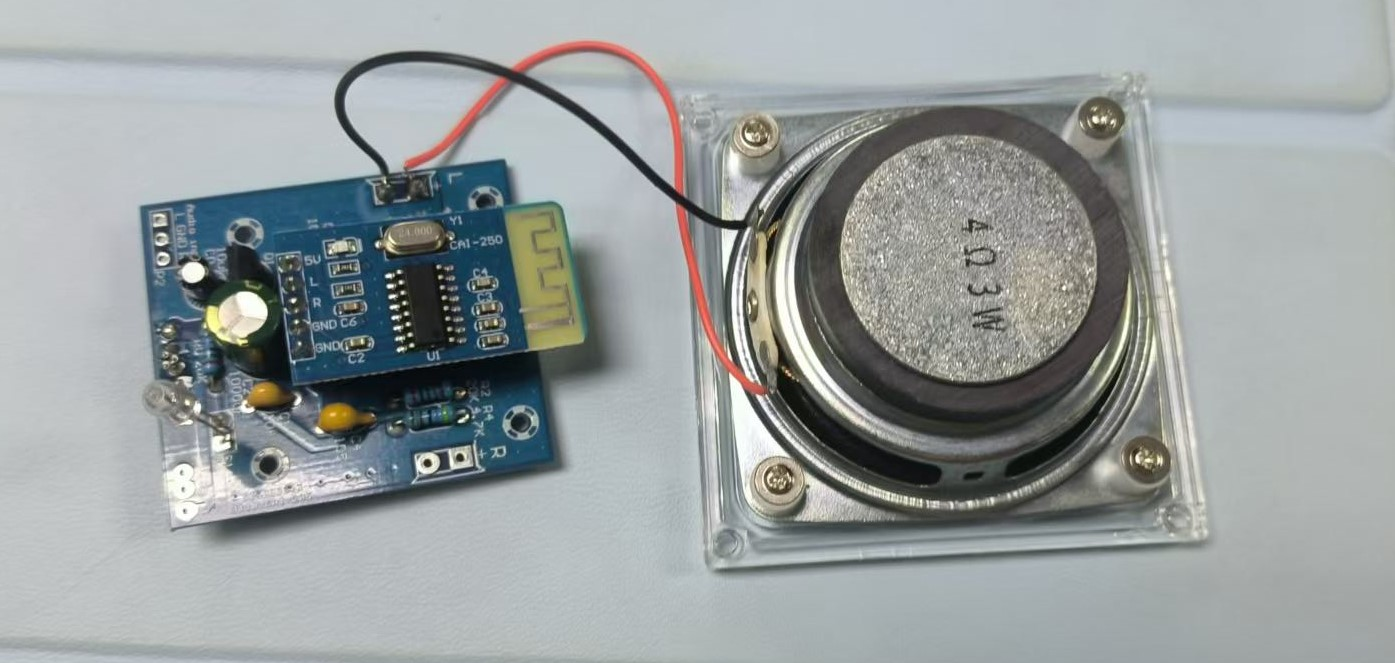
\includegraphics[width=0.5\textwidth]{ET2_1_finished_product1.jpg}
	\caption{Finished Bluetooth speaker}
	\label{fig:finished_product1}
\end{figure}

\begin{figure}[htbp]
	\centering
	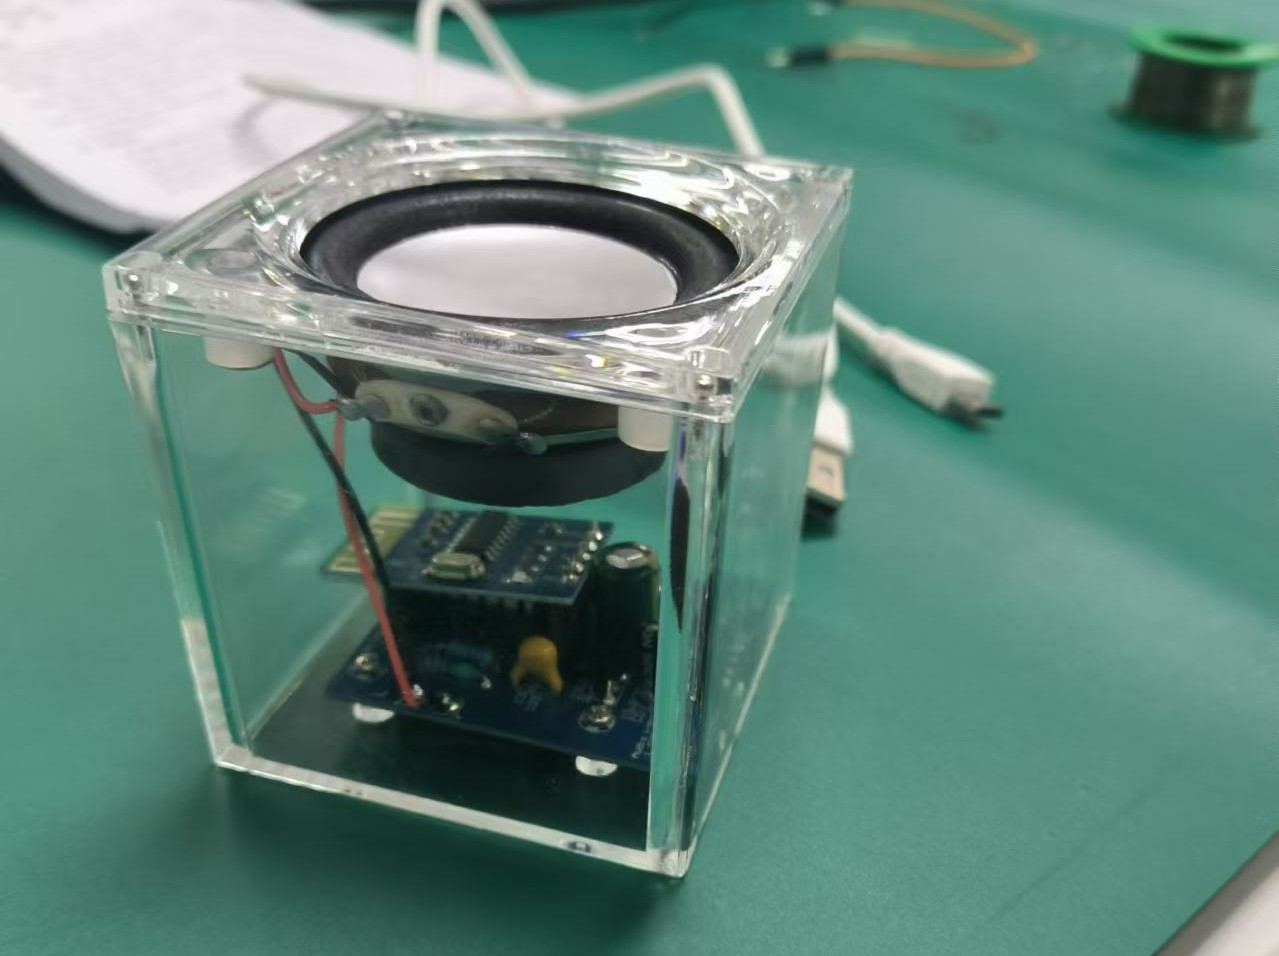
\includegraphics[width=0.5\textwidth]{ET2_1_finished_product2.jpg}
	\caption{Finished Bluetooth speaker}
	\label{fig:finished_product2}
\end{figure}

%See the \textbf{Attachment} section for the clean of the experimental bench desktop (%\cref{}).

%Other raw data are shown in %\cref{}.


%---------------------------------------------------------------------
% 问题记录
\subsection{Difficulties}
\begin{enumerate}
	\item Because it is the first time to use the soldering iron, the first class spent too much time to get familiar with the use of the soldering iron.
	\item When measuring the amplifier of the circuit, pay attention to avoid the signal generator and oscilloscope, which will lead to short circuit of the measured component, so that it can not measure the signal correctly.
	\item When measuring the magnification of the circuit, it is necessary to connect the USB power supply to provide the working voltage to the chip.
\end{enumerate}
% ---